\documentclass[master,paper]{imit-graduate}
% Кириллица без cm-super — растровая, а класс включает растяжение шрифта.
\microtypesetup{expansion=false}

\usepackage{booktabs}
\usepackage{placeins}
\graphicspath{{../../reports/ml/}{../../reports/current/}{../../reports/before/}}
\addbibresource{refs.bib}

\begin{document}
% !TEX root = main.tex
% Общие поля задания и текста ВКР. msp в классе: 01.04.02, профиль «Системное программирование».
\year{2026-2027}

\student{Синев Денис Евгеньевич
\brief Д.\,Е.\,Синев
\group М-25
\english Sinev Denis Evgenievich
}

\superviser{Секорин Всеслав Станиславович
\brief В.\,С.\,Секорин
\position доцент
\degree к.\,ф.-м.\,н.
}

\program{msp}

\title{Разработка системы мониторинга микросервисов с элементами машинного обучения
    \english Development of a microservice monitoring system with machine learning elements}

\goal{Разработка системы, которая приводит телеметрию микросервисов к единому виду, обнаруживает аномалии алгоритмом без учителя и может работать рядом с Prometheus и Zabbix.}

\begin{tasks}
\task{Реализовать ETL-конвейер для бенчмарков NAB и KPI и для промышленной телеметрии Prometheus и Zabbix: единая схема и одно признаковое пространство.
\result{Построен конвейер на Python~3.12. NAB, KPI, Prometheus и Zabbix приводятся к шести колонкам и к одним и тем же признакам ряда. Исправленный unified-прогон содержит 6\,292\,551 строку.}}
\task{Сравнить алгоритмы обнаружения аномалий без учителя на размеченных рядах при временном сплите и выбрать модель.
\result{Двенадцать детекторов сравнены на 58 рядах NAB и на восьми рядах KPI. По PR-AUC выбрана Isolation Forest: 0{,}207 на NAB и 0{,}464 на срезе KPI.}}
\task{Обучить выбранную модель и сохранить воспроизводимые артефакты.
\result{Сводка, кривые и матрицы ошибок записаны в \texttt{reports/ml}. Детектор учится отдельно на каждом ряде и не видит метку.}}
\task{Оформить сервис с конфигурируемым источником метрик и каналом оповещений.
\result{Зафиксированы контракт конфигурации, то же признаковое окно и канал webhook. Рядом уже работают конвейер \texttt{main.py} и программа сравнения \texttt{python -m ml compare}.}}
\end{tasks}


\begin{englishabstract}
The thesis builds a monitoring path for microservice telemetry.
Benchmarks NAB and KPI and industrial streams from Prometheus and Zabbix are brought to one schema.
Twelve unsupervised detectors are compared on a time-based split, and Isolation Forest is selected.
A lightweight alerting service next to the existing monitoring stack remains to be built.
\end{englishabstract}

\maketitlepage

Тема работы~--- разработка системы мониторинга микросервисов с элементами машинного обучения.
Цель~--- построить воспроизводимый путь от разнородной телеметрии до модели, которая обнаруживает аномалии и может быть поставлена рядом с существующим комплектом мониторинга (Prometheus, Zabbix).

Задачи, соответствующие этапам исследования:

\begin{enumerate}
  \item реализовать ETL-конвейер, приводящий бенчмарки и промышленную телеметрию к единой схеме и признаковому пространству;
  \item сравнить алгоритмы обнаружения аномалий без учителя на одних и тех же размеченных рядах и выбрать модель;
  \item обучить выбранную модель и сохранить воспроизводимые артефакты;
  \item оформить лёгкий сервис (контейнер) с конфигурируемым источником метрик и каналом алертов.
\end{enumerate}

Актуальность следует из того, что микросервисные системы порождают большой поток метрик, а пороги <<вручную>> плохо переносятся между сервисами и нагрузками.
Научная часть работы~--- корректная постановка эксперимента (разделение ролей датасетов, временной сплит, метрики качества) и сравнение детекторов.
Практическая часть~--- программный конвейер и последующий inference-сервис.

Структура диссертации. Глава~1 описывает источники данных и ETL.
Глава~2 фиксирует постановку эксперимента, таблицу качества двенадцати детекторов (октябрь 2026~г.) и выбор Isolation Forest.
Глава~3 описывает требования к программному продукту; контейнер рядом с Prometheus и Zabbix ещё не собран.
В заключении собраны результаты, которые уже можно защищать, и то, что остаётся до июня 2027~г.

Черновик начат в сентябре 2026~г. Официальный шаблон кафедры будет подставлен позже; содержание глав при этом сохраняется.


\chapter{Подготовка данных для обнаружения аномалий}
% !TEX root = ../main.tex
Конвейер нужен, чтобы детектор из главы~2 видел один и тот же вектор признаков и на публичном бенчмарке, и на метрике своего приложения.
Реализация~--- модульный ETL на Python~3.12.
Сырой файл остаётся в каталоге RAW, нормализованный кадр~--- в PROCESSED, итоговый набор~--- в UNIFIED.
Повторный запуск читает сырьё заново и не правит его.

\section{Источники и их роли}

В работе четыре источника.
Путать их в одной матрице нельзя: у них разные роли, и модель учится внутри одного ряда \((\texttt{source},\texttt{service},\texttt{metric\_name})\).

\begin{table}[ht]
\centering
\begin{tabular}{llp{7.2cm}}
\toprule
Источник & Метки & Роль \\
\midrule
NAB \cite{numenta-nab} & окна \(0/1\) & публичный бенчмарк \\
KPI \cite{kpi-ad} & метки организаторов \(0/1\) & основная количественная оценка \\
Prometheus \cite{prometheus} & нет (\(-1\)) & телеметрия приложения и инфраструктуры \\
Zabbix \cite{zabbix} & нет (\(-1\)) & телеметрия тестового контура \\
\bottomrule
\end{tabular}
\caption{Роли источников данных.}
\end{table}

\subsection{NAB}

Numenta Anomaly Benchmark~--- набор одномерных рядов: температура оборудования, загрузка процессора, объёмы обращений, искусственные сигналы с заранее нарисованной аномалией.
Каждый ряд лежит отдельным CSV.
Метка точки равна \(1\), если её время попадает в окно из файла \texttt{combined\_windows.json}, и \(0\) в остальных случаях.
Каталог с окнами загрузчик не читает как ряд.
В прогоне сравнения участвуют 58 CSV.

\subsection{KPI}

KPI Anomaly Detection~--- длинные операторские индикаторы.
Организаторы заранее разделили обучение и проверку: \texttt{phase2\_train.csv.gz} и \texttt{phase2\_ground\_truth.csv.gz}.
Идентификатор ряда~--- поле KPI ID.
В unified оба файла можно склеить, но для оценки модели склейка не используется: глава~2 читает их раздельно и дополнительно отбрасывает из обучения точки, которые не строго раньше первой тестовой метки того же ряда.

\subsection{Prometheus}

Prometheus уже собирает метрики приложения и машин, на которых оно стоит.
В конвейер попадают локальные parquet-дампы из \texttt{datasets/raw/PROMETHEUS/}.
Живой сервер опрашивается только если при запуске явно передан \texttt{--prom-url}.
У серии сохраняется JSON меток \texttt{job}, \texttt{instance}, \texttt{cpu}, \texttt{mode}, чтобы два одноимённых счётчика с разных машин не слиплись в один ряд.
Гистограммные ряды \texttt{*\_bucket} и служебные \texttt{*\_created} в модельный набор не берутся: это не значение сигнала, а сетка гистограммы и время создания ряда.

Годовая выгрузка приложения лежит отдельно от короткого снимка, который вошёл в unified августа 2026~г.
В каталоге \texttt{live} собрано 772 parquet.
Там есть ряды приложения (backend, bot, worker), PostgreSQL, Redis, node-exporter и проверки blackbox.
Хранение на сервере начинается с 4~августа 2026~г.
Метрики хоста берутся из node-exporter.

\subsection{Zabbix}

Zabbix тестового контура снят дампами PostgreSQL и разложен двумя parquet, потому что у истории и у трендов разный шаг.
История, \texttt{zabbix\_history.parquet}, содержит 16\,626\,504 строк.
Имя метрики~--- ключ элемента, поле \texttt{service}~--- имя хоста, метка равна \(-1\).
Тренды, \texttt{zabbix\_trends.parquet}, содержат 14\,380\,893 строк.
К ключу добавлен суффикс \texttt{\{grain="trend\_avg"\}}, значение~--- среднее за интервал тренда.
Смешивать эти два зерна в одном ряде нельзя: скользящее окно из пяти точек означало бы пять минут на истории и пять интервалов тренда на другом файле.

\section{Единая схема}

Каждый загрузчик заканчивает кадр одними и теми же колонками:
\texttt{timestamp}, \texttt{service}, \texttt{metric\_name}, \texttt{value}, \texttt{label}, \texttt{source}.
Метка принимает три значения.
\(0\)~--- норма, \(1\)~--- аномалия, \(-1\)~--- метки нет.
Precision, recall и PR-AUC считаются только по точкам \(0\) и \(1\).

Нормализация приводит время к одному типу, удаляет пустые значения и точные дубликаты и сортирует ряд по времени.
Имена метрик NAB и KPI приводятся к каноническому виду по токенам, чтобы один и тот же показатель не раздвоился из-за регистра или лишнего символа.
Ключи Zabbix и имена Prometheus не переименовываются в условные \texttt{cpu\_usage}: промышленное имя должно остаться тем, по которому оператор найдёт ряд в своей системе.

\section{Модули конвейера}

\begin{itemize}
  \item извлечение~--- \texttt{etl/loaders/}, отдельные загрузчики NAB, KPI, Prometheus и Zabbix;
  \item нормализация~--- \texttt{normalize\_dataframe()};
  \item признаки~--- скользящие статистики и разности внутри ряда;
  \item запись~--- Parquet как основной формат и CSV для просмотра;
  \item запуск~--- \texttt{etl/pipeline.py} и команда \texttt{main.py}.
\end{itemize}

Команды соответствуют источникам: \texttt{nab}, \texttt{kpi}, \texttt{prometheus}, \texttt{zabbix} и общий \texttt{all}.
Общий запуск по умолчанию читает локальные каталоги и не ходит в сеть.
Полный набор живых parquet и оба файла Zabbix в один процесс не склеиваются: такой кадр не помещается в память как единая таблица.
Для оценки моделей они и не нужны единым файлом.
Сравнение в главе~2 читает NAB и срез KPI само, минуя этот общий кадр.

\section{Признаки ряда}

После сортировки по времени для каждой точки считаются восемь признаков:
\texttt{rolling\_mean\_5}, \texttt{rolling\_mean\_15},
\texttt{rolling\_std\_5}, \texttt{rolling\_std\_15},
\texttt{rolling\_min\_5}, \texttt{rolling\_max\_5},
приращение \texttt{delta} и относительное изменение \texttt{percent\_change}.
Окно не переходит границу ряда.
В начале ряда, где истории ещё нет, пропуски признаков заполняются нулём уже в \texttt{ml\_dataset}, чтобы матрица для sklearn была плотной.

В детектор подаются исходное \texttt{value} и эти восемь колонок.
Порог по одной только величине такого вектора не видит: z-score и правило Тьюки в главе~2 специально оставлены на одной колонке \texttt{value}, чтобы было с чем сравнить методы, которые смотрят весь вектор.

\begin{figure}[ht]
\centering
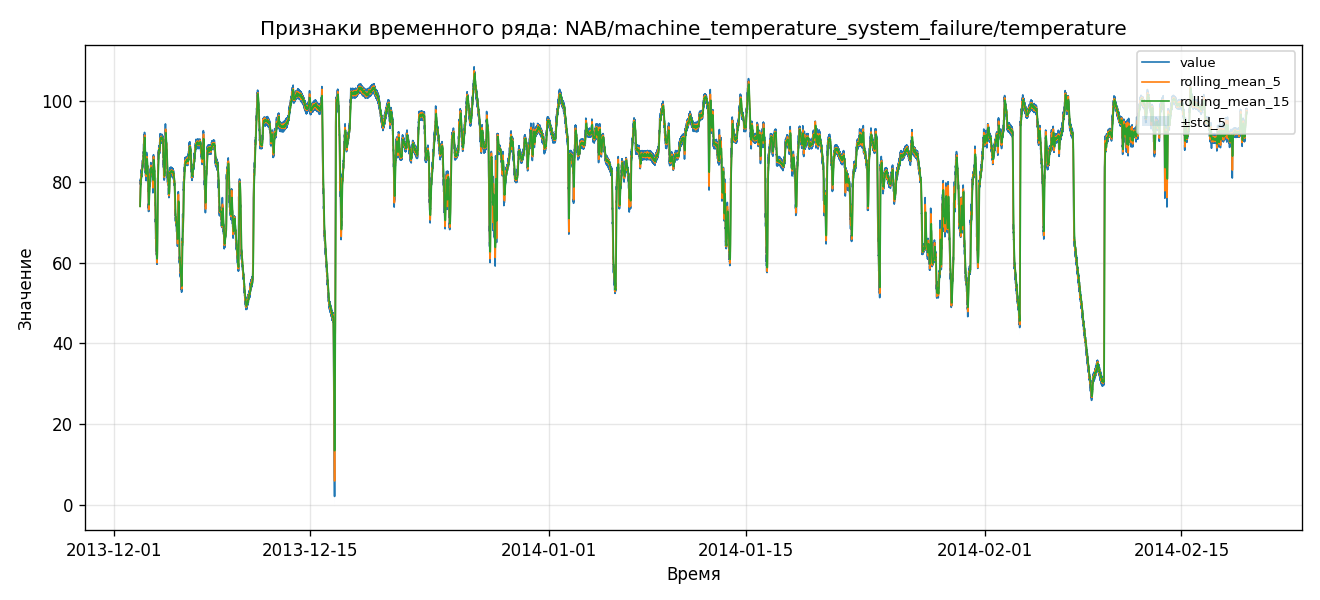
\includegraphics[width=0.92\textwidth]{NAB/features_data.png}
\caption{Ряд температуры из NAB: значение и скользящие признаки. Резкое падение видно и на среднем, и на отклонении.}
\end{figure}

На промышленном счётчике тот же расчёт выглядит иначе.
\texttt{node\_cpu\_seconds\_total} в режиме простоя растёт почти линейно: это накопительный счётчик, а не уровень загрузки.
Само значение тогда мало говорит об аномалии, а \texttt{delta} переводит его в приращение за шаг.

\begin{figure}[ht]
\centering
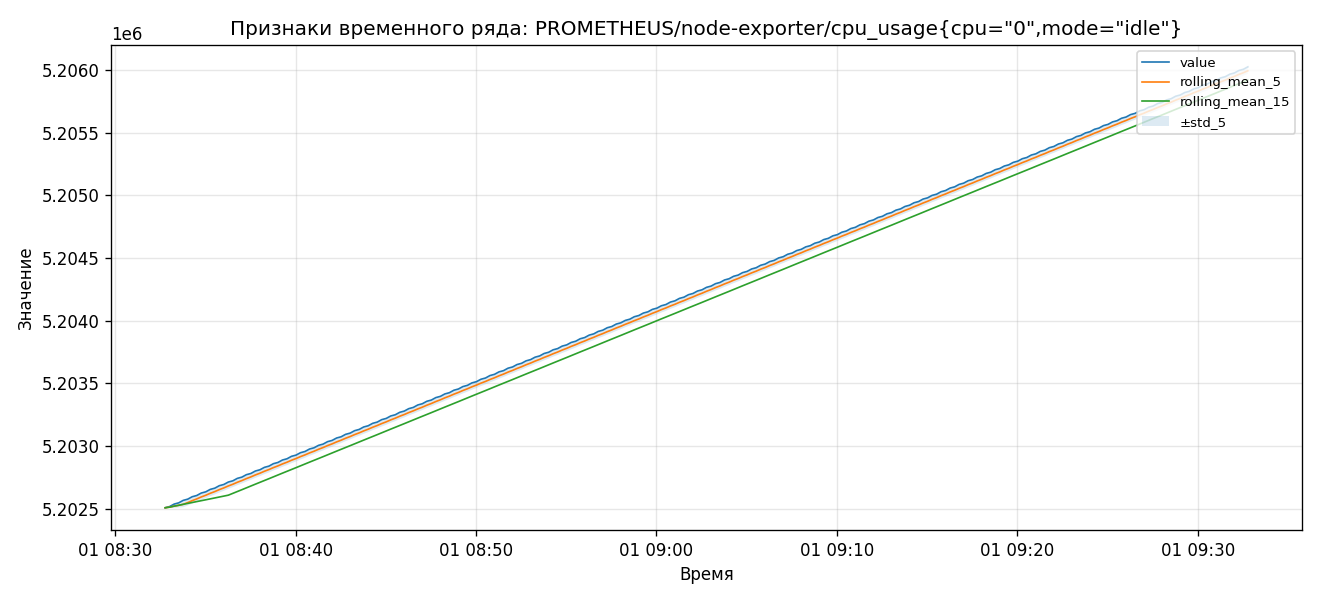
\includegraphics[width=0.92\textwidth]{PROMETHEUS/features_data.png}
\caption{Счётчик простоя CPU из node-exporter. Уровень растёт монотонно, рабочий сигнал для детектора~--- приращение.}
\end{figure}

\FloatBarrier
\section{Состав размеченного набора}

После исправления загрузчиков и привязки окон NAB полный unified-прогон дал следующий состав.
В нём короткий демонстрационный Prometheus.
Годовая выгрузка и Zabbix в этот файл не входили и лежат отдельными parquet.

\begin{table}[ht]
\centering
\begin{tabular}{lrr}
\toprule
Источник & Строк & Аномалий (\(\texttt{label}=1\)) \\
\midrule
NAB & 365\,541 & 33\,495 \\
KPI & 5\,922\,913 & 134\,114 \\
Prometheus & 4\,097 & 0 \\
\midrule
Всего & 6\,292\,551 & --- \\
\bottomrule
\end{tabular}
\caption{Состав unified-набора после исправления конвейера.}
\end{table}

Доля аномалий на NAB около \(9\,\%\), на KPI около \(2\,\%\).
На таком перекосе доля верных ответов почти ничего не говорит: детектор, который всегда отвечает <<норма>>, уже выглядит успешным.
Поэтому в главе~2 главный показатель~--- PR-AUC.

\begin{figure}[ht]
\centering
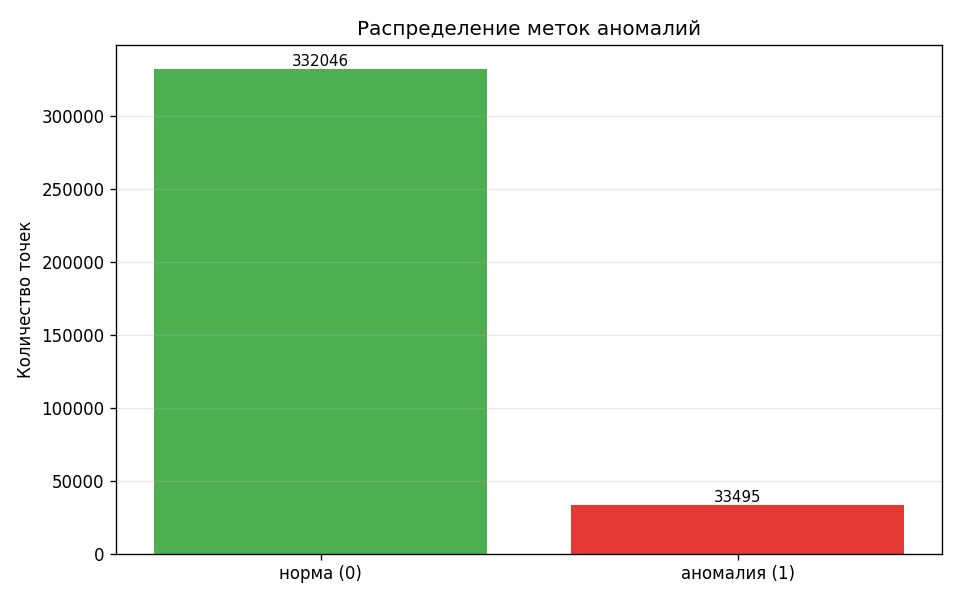
\includegraphics[width=0.78\textwidth]{NAB/anomaly_distribution.png}
\caption{Метки NAB: 332\,046 точек нормы и 33\,495 аномалий.}
\end{figure}

\begin{figure}[ht]
\centering
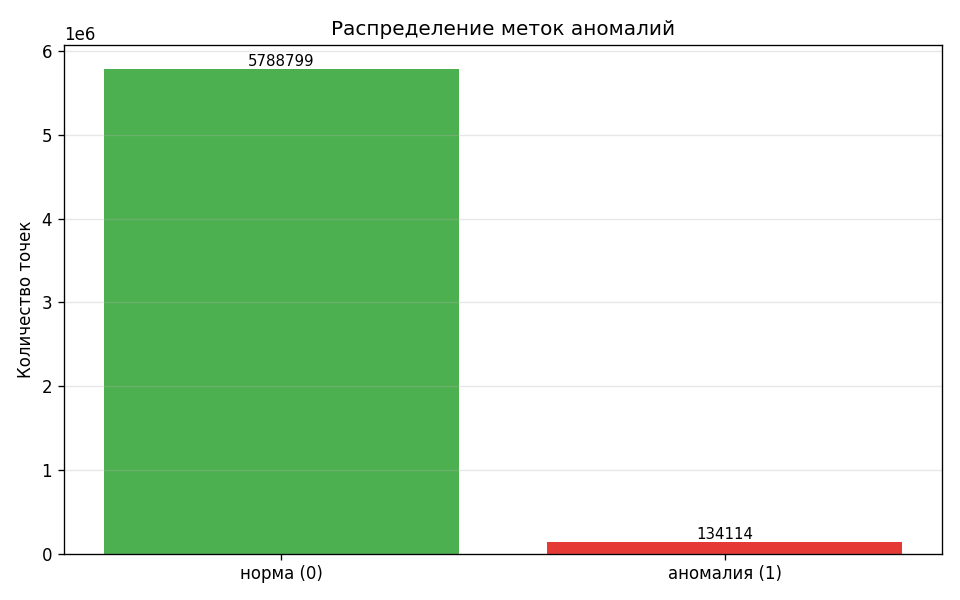
\includegraphics[width=0.78\textwidth]{KPI/anomaly_distribution.png}
\caption{Метки KPI: 5\,788\,799 точек нормы и 134\,114 аномалий.}
\end{figure}

Автотесты проверяют состав колонок, загрузчики, временной разрез и то, что в таблицу сравнения не попадают Prometheus и Zabbix.
Графики прогона конвейера пишутся в \texttt{reports/current/}.
Каталог \texttt{reports/before/} хранит снимок прежнего прогона и текущим кодом не перезаписывается.
Демонстрационный интерфейс \texttt{gui/app.py} показывает схему и уже построенные файлы.
Он не запускает загрузку и не учит модель.

\section{Что не входит в оценку качества}

Prometheus и Zabbix нужны как вход будущего сервиса и как проверка, что тот же код признаков читает промышленный ряд.
Строки качества по ним не считаются: эталона \(0/1\) нет.
Живые выгрузки в публичный репозиторий не коммитятся.
Для переноса предусмотрены архивы частями меньше 90~МБ, скрипт \texttt{scripts/pack\_datasets\_for\_git.py}.


\chapter{Сравнительное исследование моделей}
% !TEX root = ../main.tex
Сравнение выполнено одной командой, \texttt{python -m ml compare}.
Все детекторы получают один и тот же вектор из главы~1 и один и тот же временной разрез.
Метку при обучении они не видят.
Сводка лежит в \texttt{reports/ml/compare\_summary.csv}.

\section{Постановка}

Детектор anomaly detection на мониторинге нельзя учить как классификатор скоринга.
В скоринге у каждой строки есть целевая метка, и выборка перемешивается.
Здесь метка есть только у бенчмарка, а у ряда, который пойдёт в продукт, её нет.
Если перемешать время, модель увидит будущее ряда в обучении и на проверке покажет качество, которого на потоке не будет.

Для NAB обучающая часть ряда~--- точки строго до начала первого окна из \texttt{combined\_windows.json}.
Если окон нет или такая часть пуста, разрез ставится на \(70\,\%\) временного диапазона.
Проверка~--- хвост после разреза.
Для KPI обучение берётся из \texttt{phase2\_train.csv.gz}, проверка~--- из \texttt{phase2\_ground\_truth.csv.gz}.
Точки обучения, которые не строго раньше первой проверочной метки того же ряда, отбрасываются.

Главная метрика~--- PR-AUC.
Рядом считаются precision и recall по бинарному решению.
ROC строится как дополнительная картинка: на редком положительном классе она завышает впечатление от детектора, который редко ошибается на норме и пропускает почти все аномалии.
В среднее попадают только точки с меткой \(0\) или \(1\).
Prometheus и Zabbix в таблицу не входят.

Порог скоринговых моделей~--- \(97{,}5\)-й перцентиль скора на обучении данного ряда.
Z-score режет ряд по \(|z|>3\) на колонке \texttt{value}.
IQR~--- по правилу Тьюки \(1{,}5\) межквартильного размаха на той же колонке.
Эти два порога смотрят только на величину.
Остальные детекторы смотрят весь вектор и масштабируют его по обучающей части ряда.

Ансамбль имеет смысл, если детекторы ошибаются на разных типах аномалий.
Пока такого разбора нет, в продукт берётся одна модель с лучшим PR-AUC среди тех, кто учился на всём доступном ряде.

\section{Детекторы}

Обёртки собраны в \texttt{ml/models.py}.
Их двенадцать.

\subsection{Пороги по значению}

Z-score и IQR~--- бейзлайн.
Они не используют скользящие признаки.
Если лес или HBOS не обгоняют эти пороги, усложнение вектора ничего не даёт.

\subsection{Деревья, плотность и носитель}

Isolation Forest строит ансамбль случайных деревьев.
Аномалия изолируется короткой веткой, нормальная точка~--- длинной~\cite{liu2008isolation}.
LOF работает в режиме novelty: соседи считаются по обучению, проверка в построение плотности не входит~\cite{breunig2000lof}.
One-Class SVM оценивает границу носителя нормальных точек~\cite{scholkopf2001ocsvm}.
На длинном ряде он дорог, поэтому ряд с обучением длиннее 10\,000 точек пропускается.
kNN берёт расстояние до \(k\)-го соседа и пропускает ряд длиннее 20\,000 точек обучения.

\subsection{Проекция, гистограмма и расстояние}

PCA считает ошибку восстановления, не больше чем по трём компонентам.
HBOS складывает редкость точки по гистограмме каждой координаты, по десять корзин~\cite{goldstein2012hbos}.
Расстояние Махаланобиса берётся от эмпирического среднего и ковариации обучающей части.
К ковариации добавляется малая диагональ, чтобы матрица не разваливалась на коротком ряде.
Elliptic Envelope оценивает робастную ковариацию не больше чем по 8\,000 случайным точкам.
Если оценка не сходится, обёртка подставляет расстояние Махаланобиса.
В таблице длина обучения для этой модели всё равно указана полностью.

\subsection{Плотность и кластеры}

Одна гауссиана, GMM, даёт скор как минус логарифм плотности.
k-means строит до четырёх центров, скор~--- расстояние до ближайшего.
Оба метода описывают <<типичное>> положение ряда и поднимают скор там, где точка от него ушла.

Короткий прогон на трёх рядах NAB в выбор не идёт.
На нём впереди оказывался LOF.
Ниже приведён полный прогон.

\section{Состав прогона}

NAB: все 58 CSV, 135\,755 точек обучения и 229\,803 точки проверки у моделей без ограничения длины.
У One-Class SVM один ряд длиннее порога, поэтому у него 119\,204 и 228\,304 точки.

Полный KPI в память не загружается: в файлах около 3{,}0~млн строк обучения и 2{,}9~млн строк проверки.
Берутся первые восемь идентификаторов из отсортированного пересечения двух файлов: 822\,319 и 798\,580 точек.
Список идентификаторов записан в \texttt{reports/ml/kpi\_slice\_ids.txt}.
На проверке этого среза 10\,607 аномалий, что видно по матрице ошибок леса ниже: \(9224 + 1383\).

\FloatBarrier
\section{NAB}

Цифры округлены до трёх знаков.
Исходный файл не округлялся.

\begin{table}[ht]
\centering
\small
\begin{tabular}{lrrr}
\toprule
Модель & PR-AUC & Precision & Recall \\
\midrule
z-score & 0{,}182 & 0{,}295 & 0{,}116 \\
IQR & 0{,}187 & 0{,}260 & 0{,}204 \\
Isolation Forest & 0{,}207 & 0{,}194 & 0{,}399 \\
LOF & 0{,}171 & 0{,}195 & 0{,}286 \\
One-Class SVM & 0{,}161 & 0{,}185 & 0{,}308 \\
kNN & 0{,}191 & 0{,}243 & 0{,}265 \\
PCA & 0{,}189 & 0{,}231 & 0{,}180 \\
HBOS & 0{,}206 & 0{,}253 & 0{,}201 \\
Махаланобис & 0{,}199 & 0{,}262 & 0{,}221 \\
Elliptic Envelope & 0{,}185 & 0{,}223 & 0{,}157 \\
GMM & 0{,}198 & 0{,}262 & 0{,}221 \\
k-means & 0{,}195 & 0{,}254 & 0{,}233 \\
\bottomrule
\end{tabular}
\caption{NAB, 58 рядов. У One-Class SVM на один ряд меньше.}
\end{table}

\begin{figure}[ht]
\centering
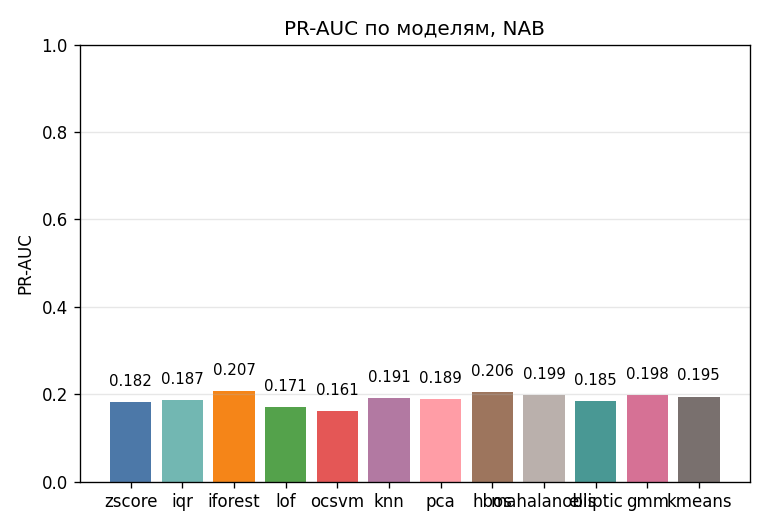
\includegraphics[width=0.92\textwidth]{pr_auc_bars_NAB.png}
\caption{PR-AUC на NAB. Isolation Forest и HBOS стоят рядом, остальные ниже.}
\end{figure}

Абсолютные значения на NAB низкие: лучший результат \(0{,}207\).
Отрыв леса от HBOS (\(0{,}206\)) на этом бенчмарке маленький.
Оба всё же выше порогов по одному значению.
Матрица ошибок леса на NAB показывает ту же картину, что и recall \(0{,}40\): заметная доля аномалий остаётся в столбце нормы.

\begin{figure}[ht]
\centering
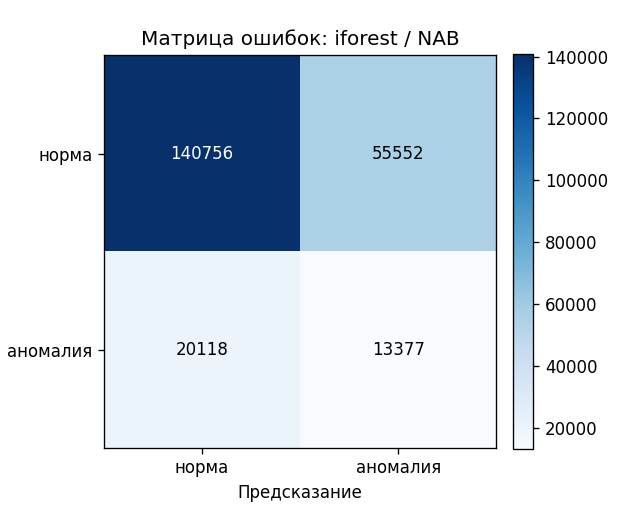
\includegraphics[width=0.72\textwidth]{cm_NAB_iforest.png}
\caption{Матрица ошибок Isolation Forest на NAB.}
\end{figure}

\FloatBarrier
\section{KPI}

\begin{table}[ht]
\centering
\small
\begin{tabular}{lrrr}
\toprule
Модель & PR-AUC & Precision & Recall \\
\midrule
z-score & 0{,}176 & 0{,}649 & 0{,}061 \\
IQR & 0{,}270 & 0{,}391 & 0{,}216 \\
Isolation Forest & 0{,}464 & 0{,}112 & 0{,}870 \\
LOF & 0{,}173 & 0{,}280 & 0{,}283 \\
PCA & 0{,}257 & 0{,}228 & 0{,}544 \\
HBOS & 0{,}355 & 0{,}363 & 0{,}465 \\
Махаланобис & 0{,}385 & 0{,}245 & 0{,}583 \\
Elliptic Envelope & 0{,}354 & 0{,}257 & 0{,}587 \\
GMM & 0{,}374 & 0{,}245 & 0{,}583 \\
k-means & 0{,}378 & 0{,}285 & 0{,}607 \\
\bottomrule
\end{tabular}
\caption{KPI, восемь рядов, полное обучение (822\,319 / 798\,580 точек).}
\end{table}

One-Class SVM и kNN на этом срезе посчитаны только по двум коротким рядам, по 17\,568 точек с каждой стороны.
Их PR-AUC, \(0{,}418\) и \(0{,}383\), в таблицу выше не поставлены: это другой объём данных.
На столбчатой диаграмме они видны, и подпись к рисунку это оговаривает.

\begin{figure}[ht]
\centering
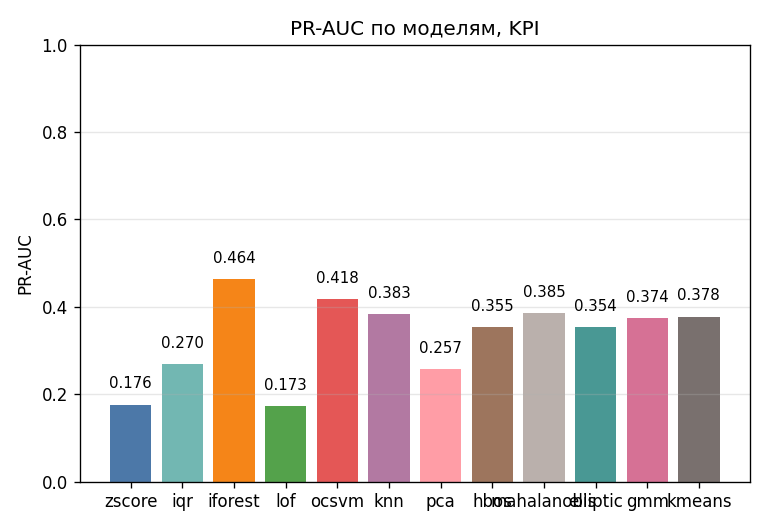
\includegraphics[width=0.92\textwidth]{pr_auc_bars_KPI.png}
\caption{PR-AUC на срезе KPI. Столбцы One-Class SVM и kNN относятся к двум коротким рядам.}
\end{figure}

\begin{figure}[ht]
\centering
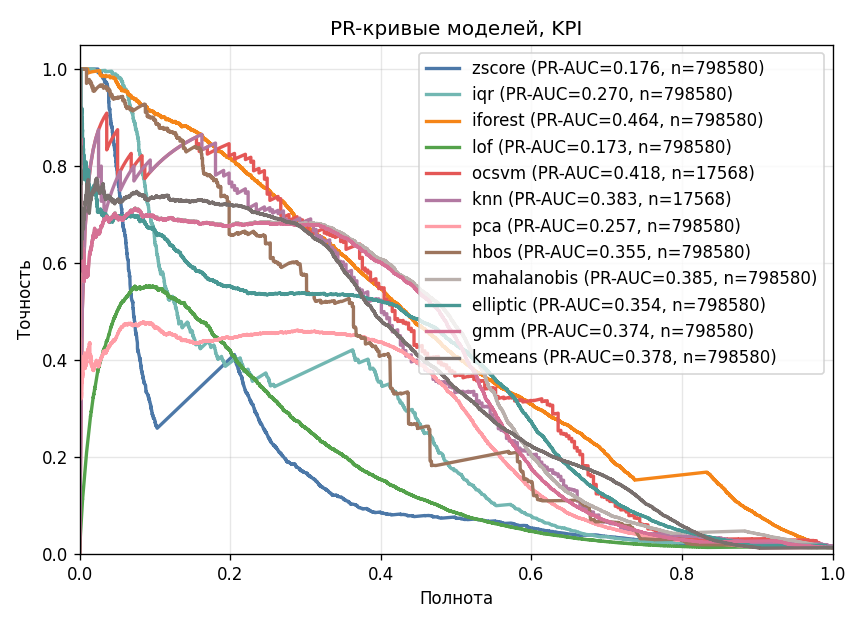
\includegraphics[width=0.92\textwidth]{pr_curves_KPI.png}
\caption{Кривые precision--recall на срезе KPI. Кривая леса дольше держит полноту.}
\end{figure}

\begin{figure}[ht]
\centering
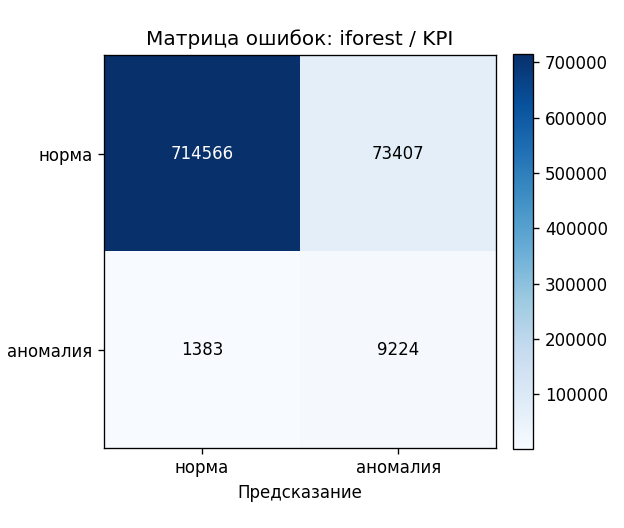
\includegraphics[width=0.72\textwidth]{cm_KPI_iforest.png}
\caption{Матрица ошибок Isolation Forest на срезе KPI: 9\,224 найденные аномалии, 1\,383 пропуска и 73\,407 ложных тревог.}
\end{figure}

\begin{figure}[ht]
\centering
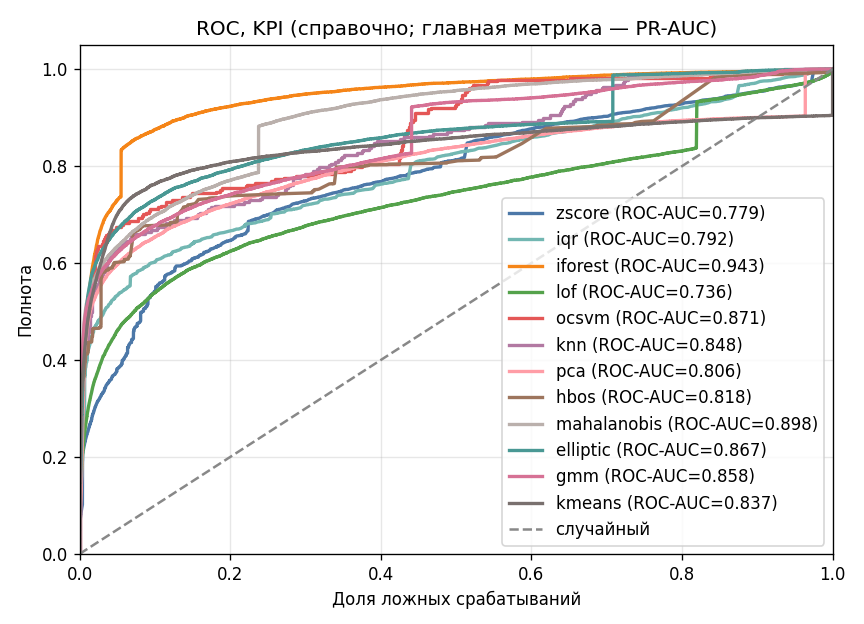
\includegraphics[width=0.88\textwidth]{roc_curves_KPI.png}
\caption{ROC на срезе KPI. Кривые сжимаются в левый верхний угол слабее, чем различается PR-AUC, поэтому выбор сделан по PR-AUC.}
\end{figure}

\FloatBarrier
\section{Выбор модели}

Для продукта берётся Isolation Forest.
На обоих размеченных источниках у него лучший PR-AUC среди моделей, которые учились на всём ряде: \(0{,}207\) на NAB и \(0{,}464\) на срезе KPI.

На KPI у леса полнота \(0{,}87\) и точность \(0{,}11\).
Из 10\,607 аномалий пропущены 1\,383, ложных тревог 73\,407.
Z-score на том же срезе почти не ошибается в положительном классе (precision \(0{,}65\)), но полнота \(0{,}06\): он молчит.
Для мониторинга пропуск аномалии дороже лишнего сигнала, поэтому рабочая точка леса полезнее.
Порог \(97{,}5\)-го перцентиля можно сдвинуть, когда появится контур оповещения и станет ясно, сколько тревог оператор готов разбирать.

Следующие по полному обучению на KPI: расстояние Махаланобиса (\(0{,}385\)), k-means (\(0{,}378\)), GMM (\(0{,}374\)), HBOS (\(0{,}355\)).
Они остаются в главе как фон сравнения.
Отдельный файл \texttt{detector.joblib} под один глобальный ряд не записывался: детектор учится на каждом ряде заново, и для сервиса нужен тот же режим, а не одна матрица на все метрики сразу.


\chapter{Программная система мониторинга}
% !TEX root = ../main.tex
Программа работы состоит из двух уже запускаемых частей и одного контракта поставки.
Первая часть готовит данные, вторая сравнивает детекторы и сохраняет таблицу с рисунками.
Контракт описывает, как выбранный лес ставится рядом с уже работающим мониторингом.

\section{Состав}

Код разделён так, чтобы сравнение моделей не тащило за собой загрузку всех промышленных дампов.

\begin{itemize}
  \item \texttt{etl/}~--- загрузчики, нормализация, признаки, схема шести колонок;
  \item \texttt{main.py}~--- команды \texttt{nab}, \texttt{kpi}, \texttt{prometheus}, \texttt{zabbix}, \texttt{all};
  \item \texttt{ml/}~--- разрез по времени, двенадцать детекторов, метрики, рисунки, команда сравнения;
  \item \texttt{gui/app.py}~--- просмотр схемы и уже построенных файлов;
  \item \texttt{reports/ml/}~--- сводка и рисунки главы~2;
  \item \texttt{reports/current/}~--- рисунки прогона конвейера.
\end{itemize}

Зависимости ставятся в виртуальное окружение Python~3.12.
Системный интерпретатор дистрибутива для прогона не используется.

\section{Конвейер}

Запуск без аргументов источника читает локальные каталоги \texttt{datasets/raw/}.
Prometheus по умолчанию не обращается к HTTP.
Адрес живого сервера передаётся флагом \texttt{--prom-url} вместе со списком PromQL.
Флаг \texttt{--no-viz} отключает рисунки, если нужен только кадр данных.

Общая команда \texttt{python main.py all} собирает единый набор из тех источников, которые переданы явно или берутся из каталогов по умолчанию.
Готовый \texttt{ml\_dataset} содержит \texttt{value} и восемь признаков главы~1 без пропусков.
Этот файл удобен для проверки схемы.
Полное сравнение моделей его не ждёт: NAB читается своими CSV, KPI~--- потоком по выбранным идентификаторам.
Так длинный файл KPI не поднимается в память целиком.

\section{Программа сравнения}

Команда \texttt{python -m ml compare} повторяет протокол главы~2.
Она обходит ряды, учит каждый детектор на прошлом участка ряда, считает PR-AUC, precision и recall на хвосте и пишет PNG.
Отдельные флаги ограничивают прогон одним источником или меняют число рядов KPI.
Идентификаторы среза сохраняются рядом со сводкой, чтобы таблицу можно было повторить.

На выходе для каждого источника и каждой модели есть матрица ошибок и кривая precision--recall.
Поверх них строятся общие кривые PR и ROC и столбцы PR-AUC.
Именно эти файлы стоят в главе~2.
Повторный запуск перезаписывает каталог \texttt{reports/ml/} и не трогает \texttt{reports/before/}.

Детектор в этом режиме не сериализуется в один файл на все ряды.
У каждого ряда своё обучение.
Для сервиса это же правило: окно последних точек конкретной метрики, \texttt{fit} на этом окне или уже посчитанный масштаб ряда, затем скор новой точки.
Общая матрица <<на все сервисы сразу>> противоречила бы разрезу, на котором лес обогнал остальные методы.

\section{Просмотр результатов}

Интерфейс \texttt{gui/app.py} нужен, чтобы открыть схему конвейера и посмотреть уже сохранённые рисунки, не запуская обучение из браузера.
Он не заменяет команду сравнения и не ходит в Prometheus.
Для защиты и для повторения чисел достаточно каталога \texttt{reports/ml/} и команды из раздела выше.

\section{Сервис рядом с мониторингом}

Целевая поставка~--- контейнер без интерфейса и без прогона миллионов строк.
Источник задаётся файлом, а не правкой кода.
Признаки те же, что в ETL, и считаются по короткому окну последних точек.
Решение отдаётся webhook-запросом в канал, который уже принят в контуре.

\begin{verbatim}
source:
  type: prometheus   # или zabbix
  url: http://prometheus:9090
  scrape_interval_sec: 30
  queries: [...]
sink:
  type: webhook
  url: https://example.invalid/alert
model:
  path: /models/detector.joblib
  window: 15
\end{verbatim}

Zabbix подключается вторым коннектором в ту же схему из шести колонок.
История и тренды остаются разными рядами, как в главе~1.
Файл \texttt{detector.joblib} в репозитории ещё не собран: сравнение выбирает алгоритм и сохраняет таблицу с рисунками, а упаковка леса в этот путь~--- шаг поставки контейнера.
Порог тревоги остаётся параметром сервиса.
На KPI текущая точка леса ловит \(87\,\%\) аномалий среза ценой низкой точности, и для конкретного канала её можно поднять.


\conclusion
% !TEX root = ../main.tex
На октябрь 2026~г. выполнены первые два этапа работы.

ETL приводит NAB, KPI, Prometheus и Zabbix к схеме из шести колонок и к одному набору признаков по каждому ряду.
Разметка NAB и KPI исправлена; в текст входят цифры прогона августа 2026~г. (6\,292\,551 строк unified), а не числа сломанного отчёта НИР-1.
Живые выгрузки лежат отдельно: 772 parquet Prometheus и два parquet Zabbix (16\,626\,504 строк истории и 14\,380\,893 строк трендов).
У этих точек метка $-1$, поэтому они не входят в таблицу качества.

Двенадцать детекторов без учителя сравнены на 58 рядах NAB и на восьми рядах KPI при временном сплите.
По PR-AUC на полном обучении выбран Isolation Forest ($0{,}207$ на NAB и $0{,}464$ на срезе KPI).
One-Class SVM и kNN на KPI посчитаны только на двух коротких рядах, и этот результат в выбор модели не входит.

Дальше: сохранить выбранный лес, построить лёгкий контейнер с тем же признаковым окном и с конфигурируемым источником Prometheus или Zabbix, и отдельно посмотреть, дополняют ли HBOS и расстояние Махаланобиса ошибки леса.
Качественные графики на рядах без эталона остаются приложением к промышленной части, а не строкой PR-AUC.


\printthebibliography
\end{document}
